\chapter{Interoperability}
\section{Syntactic}
Interoperability is the ability of making systems and organizations work together or inter-operate. When talking about information systems the syntactic interoperability is the first step.
One system cannot recieve any data in a format it does not accept, although this probably is self explanatory, it should be mentioned.
The level of ineffectiveness is enourmous because of this simple problem. I would first relate this to switching-costs and lock-in for users. As of now there is 3 main operating systems, Linux, Windows and OSX. Businesses would have to think twice before deciding on either. First one would have to train personell to use the operating system, so one would be subject to brand-specific-training lock-in \cite{15}. This in turn would make the use of the system a barrier for interoperability, since users are now trained in one operating system and would now prefer this over the others. Now, some software is only supported for some operating systems, or OS's\nomenclature{OS's}{Operating Systems}. If one relies on one OS, then uses software that is only supported by this OS, chances are that it would be problematic to exchange information to a different OS. The first thing to consider is that the data representation is likely to be very different from software to software. 
\begin{figure}
\centering
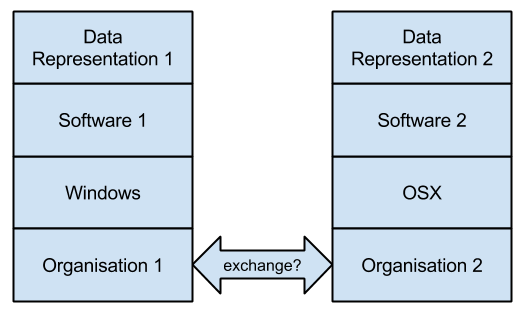
\includegraphics[width=12cm]{litterature/images/begin_silo}
\label{begin_silo}
\caption{The beginning of Silos}
\end{figure}
Just to illustrate the problem, let's say one organisation is running Windows as in in figure \ref{begin_silo} and another running OSX. The users of each organisation has had training on the operating system of their organisation, making the switching costs substantial. Money is already been invested in software that only runs on the given OS and the data representation is only supported by the software running on the OS. Clearly they would have some work to do before being able to exchange data. This type of scenario represents the formation of silos. Silos are systems which are closed to the outside. These systems have trouble with exchanging data with external systems. 

\section{Semantic}
Another part of interoperabillity is semantic interoperability. In this case the problem will be more subtle.
The syntax is the same, but the meaning behind it is different. 
A simple example like when two people are asked to work together. Both understand what it means, but have different understandings on how to do it.
Person one will split the work in half an take his share. Person two is constantly askiing person one about his half and sharing ideas on how to do it.
When they finish, person one is complaining on how he would have to do almost all the work for both of them. Person two is complaining that person one was reluctant to work together. 
This exemplefies how different semantics would make less likely for these two individuals to work together in the future, thus decreasing the level of interoperability. Of course in the computer world it would not be that easy to find out if all parties involved are understanding it the same way.


\section{Solutions and methods}
To achieve interoperability between systems one has to integrate one with the other systems in the same environment or context.
Systems in the same context is the same as systems in the same bubble. It's just a way to refine our model so we don't have take all systems in the world into account. 
The general approach to achieving interoperability is to define a common standard between systems. Through these standard channels the system would be able to communicate with echother. 
I will present four general approaches here that are loosely defined\cite{16}. 
\begin{description}
\item[Vertical integration]In this approach we do consider the different systems as silos. 
Each of the silos contributes with some functionality and as a whole delivers the required functionality.
This would probably provide the cheapest solution for gaining interoperability short-term.
\item[Star integration]Each system has a one interface for all other systems. Thus, introducing a new system would be quite expensive since one would have to make an interfaces for all existing systems. This method does make it easy to reuse functionality between systems. 
\item[Horizontal integration]In this approach one uses a own system dedicated to facilitate communication between systems. This way only one more interface is needed when introducing a new system.
\item[Common data format]This method only requires that one sets a standard data exchange format. It is recommended to provide an adapter so that one could easily transform from the native format to the common bus format. 
\end{description}
Of course this just exemplefies how to go about interoperability, as mentioned above, the general approach is to agree of a standard way of communicating cross systems. 
\section{Experiences}
To give an estimate of the benefits of interoperability I would like to re-present some data collected and analyzed by a group of scientists in the USA\cite{11}.
\begin{figure}
\centering
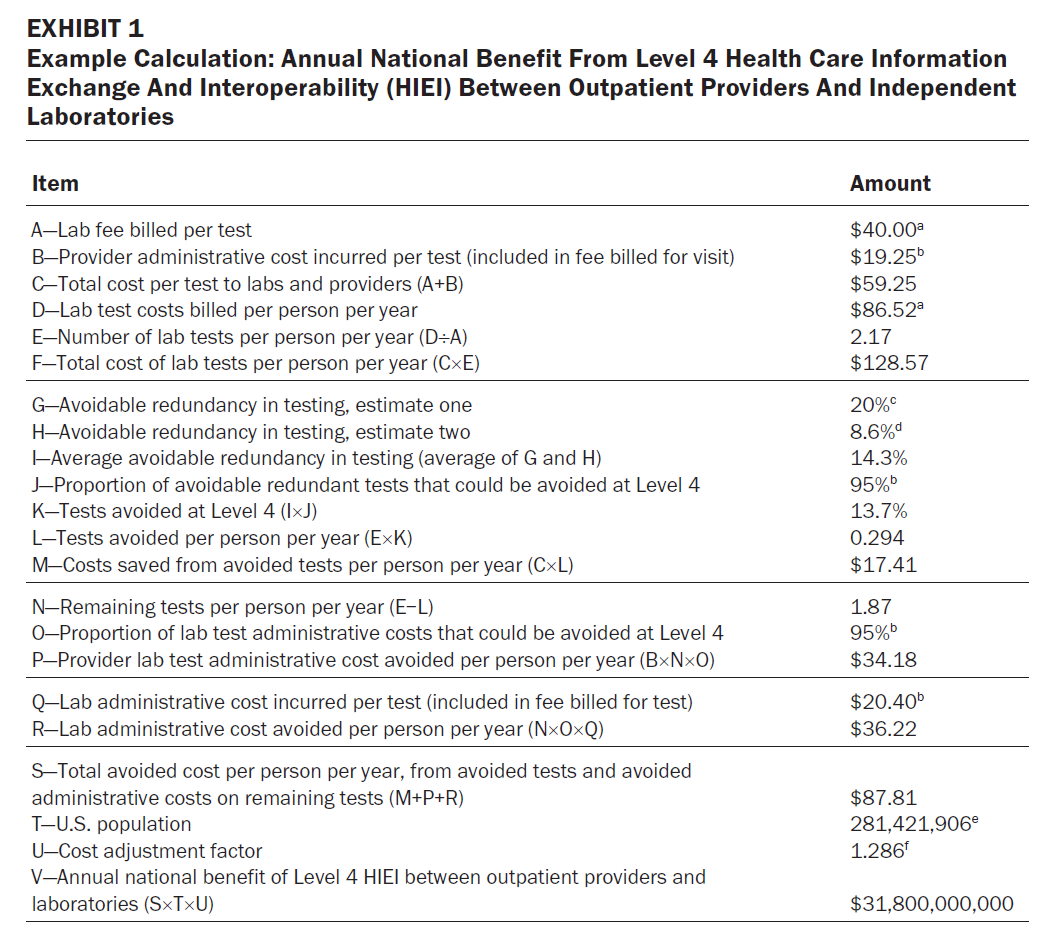
\includegraphics[width=12cm]{litterature/images/exhibit1}
\caption{Exhibit 1}
\label{fig:exhibit_1}
\end{figure}
\begin{figure}
\centering
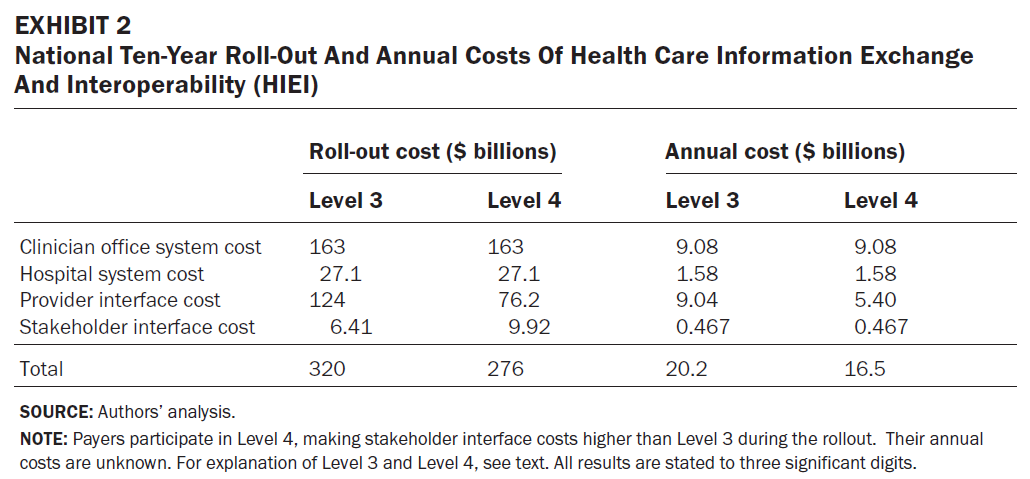
\includegraphics[width=12cm]{litterature/images/exhibit2}
\caption{Exhibit 2}
\label{fig:exhibit_2}
\end{figure}
These numbers are based on upgrading the health information system in USA.
The financial gain in figure \ref{fig:exhibit_1} represents the annual gain by upgrading to a system described below.
\begin{quote}
Machine-interpretable data—transmission of structured messages containing standardized and coded data; idealized state in which all systems exchange information using the same formats and vocabularies (examples: automated exchange of coded results from an external lab into a provider’s EMR, automated exchange of a patient’s “problem list”).
\end{quote}
This is what they call level 4. Figure \ref{fig:exhibit_2} describes the estimated costs for such a system. As one would notice the roll-out costs are substantial, but looking forward stakeholders would probably begin harvesting from their investment withing a decade. 
Also, not all benefits can be measured in terms of money. The possibilities for new technology to make its appearance is huge. The reduction of error, ease of improving data exchange with other sectors in society and the possibility of reusing functionality should also be considered when measuring the benefits of interoperability.